\section{Analisi cinetostatica}
Una volta effettuata la cinematica e dinamica del sistema in questo capitolo andiamo a presentare l'analisi cinetostatica attraverso gli ellissoidi di manipolabilità. In particolare andremo a concentrarci sui punti di singolarità, sul numero di condizionamento e per concludere andremo ad analizzare lo spazio di lavoro del manipolatore.
\begin{figure}[ht]
	\begin{center}
		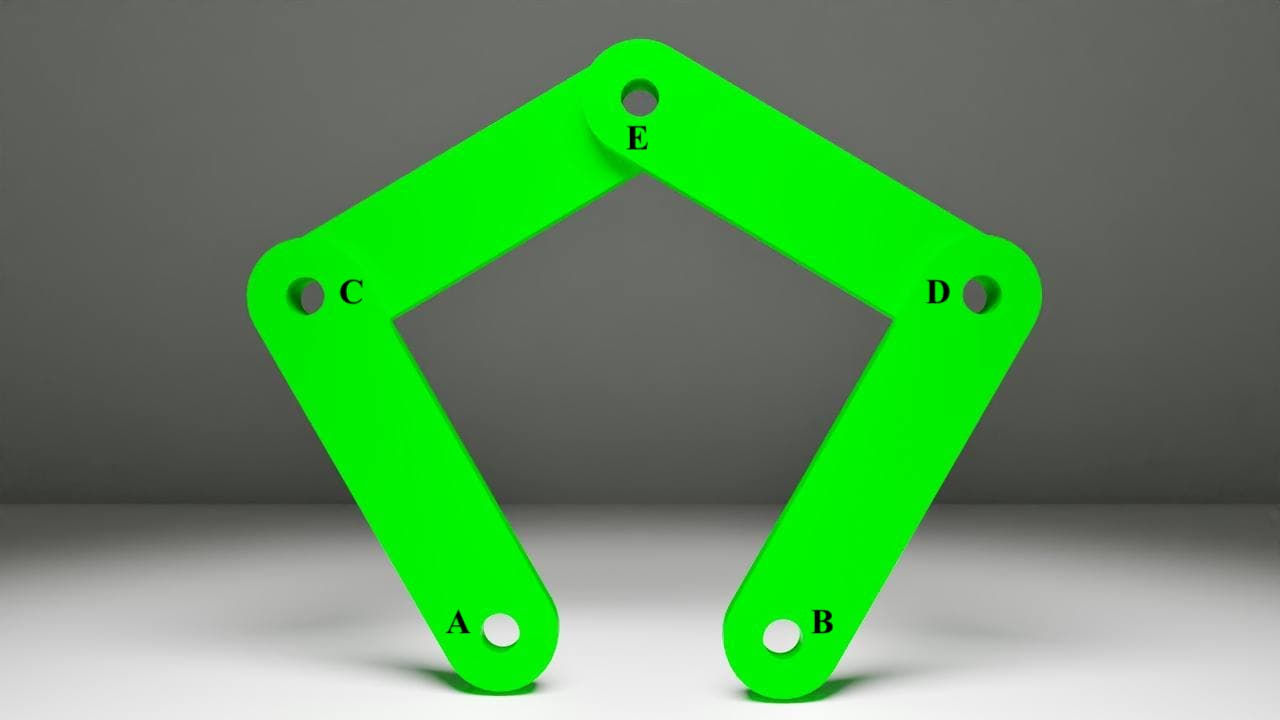
\includegraphics[scale=0.4]{Immagini/Singolarity/0}
		\caption{Posizione standard manipolatore}
	\end{center}
\end{figure}
\subsection{Punti di singolarità}
Nell'ambito matematico, una singolarità è un punto nel quale un oggetto non è definito, oppure un punto nel quale l'oggetto non ha un comportamento normale, nel nostro caso i punti di singolarità saranno punti che andranno a delimitare lo spazio di lavoro del robot. Definiamo spazio di lavoro del robot tutto un insieme di punti nei quali il robot ha un funzionamento normale e non presenta problematiche.\footnote{Passando per un punto di singolarità il robot potrebbe aver problemi che potrebbero causare anche la rottura di parti meccaniche} Andando a considerare la foto vista nell'introduzione, possiamo trovare sei casi di punti di singolarità, in particolare però non sono punti ma sono traiettorie. Di conseguenza il robot avrà come spazio di lavoro, tutto lo spazio che è interno (delimitato) da queste traiettorie.
\subsubsection*{Primo e secondo caso}
\addcontentsline{toc}{subsubsection}{Primo e secondo caso}
In questo primo caso abbiamo $\overrightarrow{CD}$ che è parallelo a $\overrightarrow{DE}$, schematicamente possiamo andarlo a rappresentare nel seguente modo
\begin{figure}[ht]
	\begin{center}
		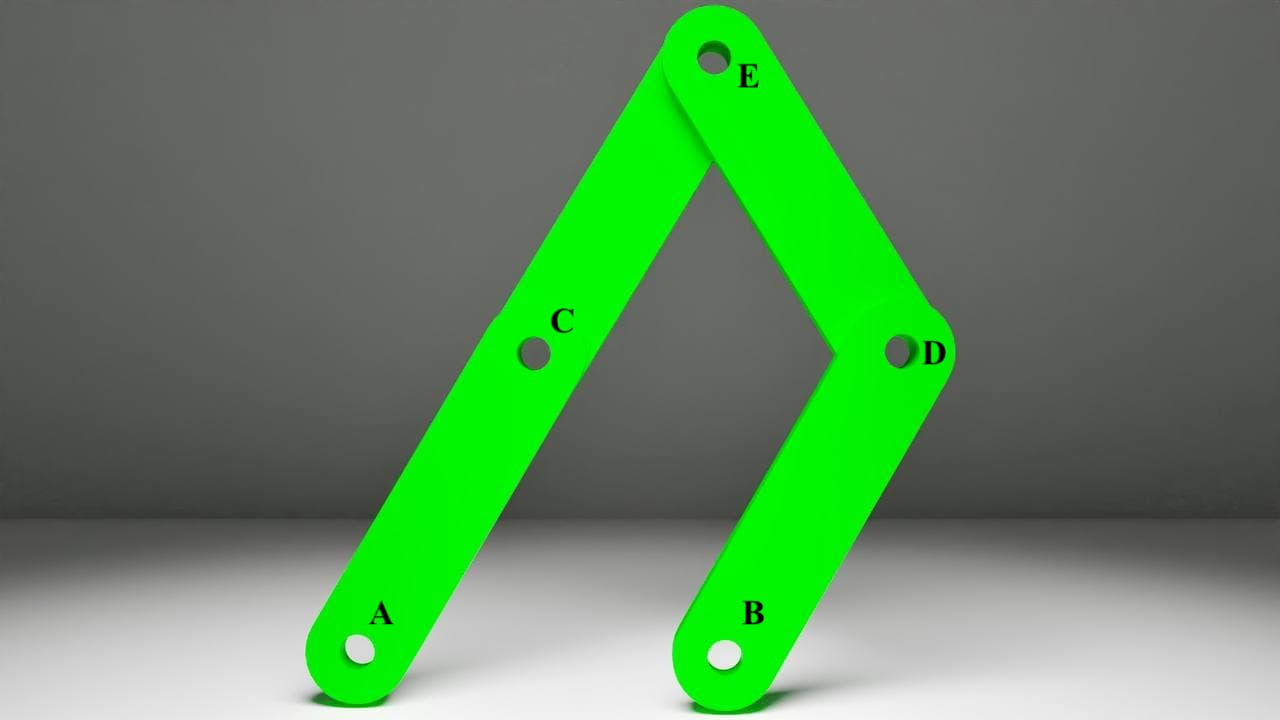
\includegraphics[scale=0.4]{Immagini/Singolarity/1}
		\caption{Caso 1 singolarità}
	\end{center}
\end{figure}
\\Lasciando la x libera possiamo ricavare la y come:
\begin{equation}
    y_1 = \sqrt{4l^2-(x-d)^2}
\end{equation}
Per quanto riguarda il secondo caso è molto simile al primo, la differenza sta nel fatto che abbiamo la catena $\overrightarrow{AB}$ parallela a $\overrightarrow{BC}$ 
\begin{figure}[ht]
	\begin{center}
		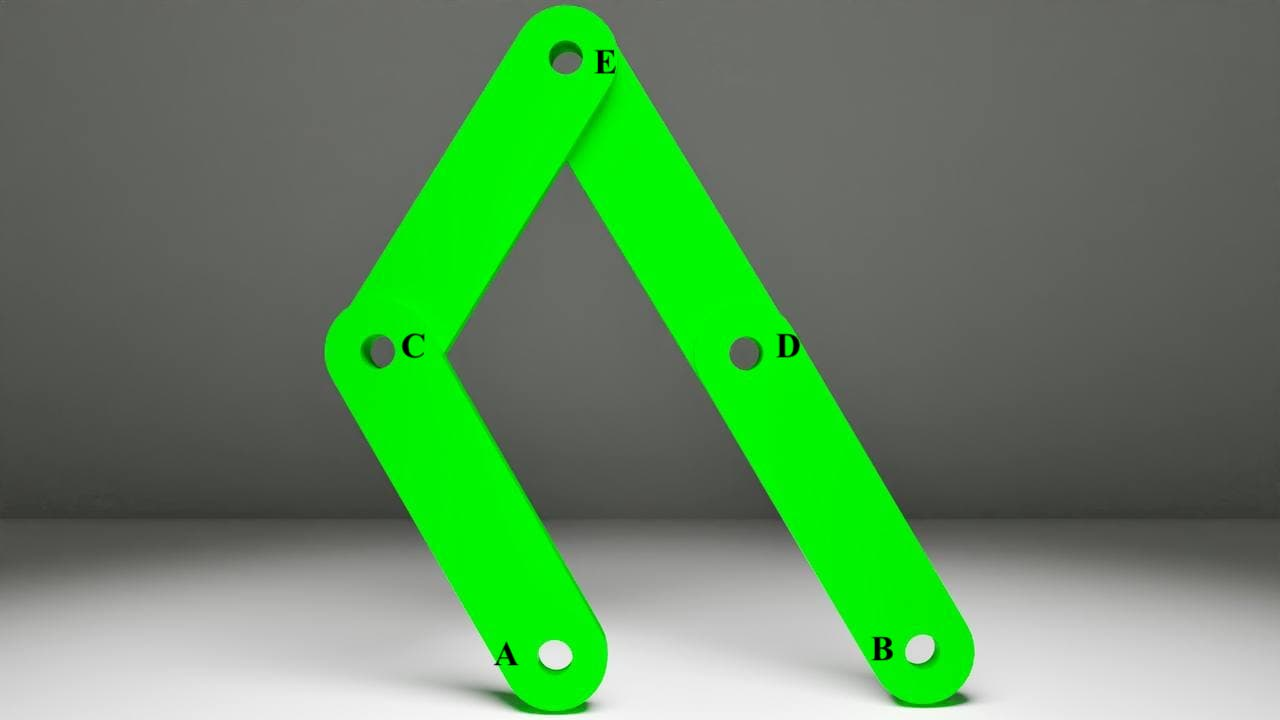
\includegraphics[scale=0.4]{Immagini/Singolarity/2}
		\caption{Caso 2 singolarità}
	\end{center}
\end{figure}
Il procedimento è simile a prima, lasciando sempre la x libera possiamo trovare la y come:
\begin{equation}
    y_2 = \sqrt{4l^2-(x+d)^2}
\end{equation}
Entrambi i casi producono come risultato una circonferenza.
\subsubsection*{Terzo caso}
\addcontentsline{toc}{subsubsection}{Terzo caso}
Il terzo caso di singolarità avviene quando i due link non motorizzati sono paralleli, questa configurazione aggiunge un grado di libertà al sistema, in quanto l'end-effector per muoversi ha necessità di una maggior coppia per riuscire a superare la situazione di stallo
\begin{figure}[ht]
	\begin{center}
		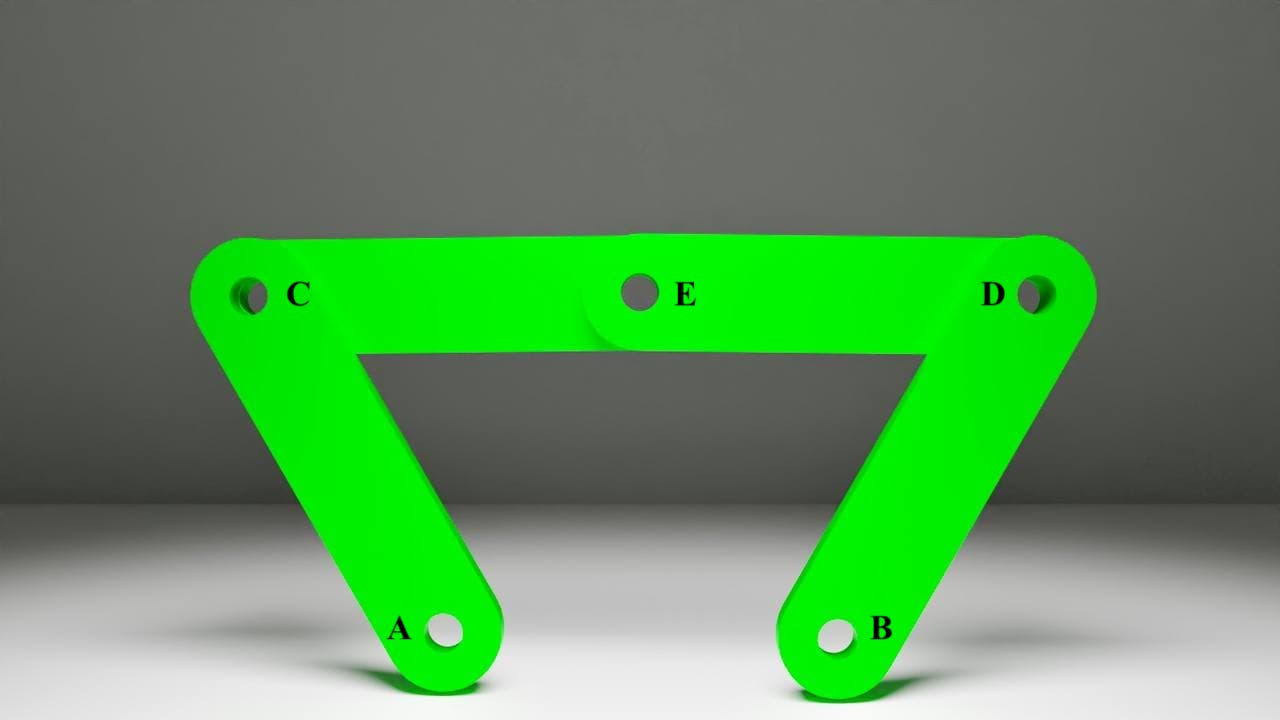
\includegraphics[scale=0.4]{Immagini/Singolarity/5}
		\caption{Caso 3 singolarità}
	\end{center}
\end{figure}
\\Per quanto riguarda la soluzione, andiamo a considerare $\theta_1$ che varia da 0 a $360^\circ$ e andiamo a cercare le coppie di valori $[x,y]$ relative alla singolarità. Uscirà un'equazione di secondo grado, con i seguenti coefficienti:
\begin{equation*}
	a = l^2\sin^2\theta_1 + 4d^2-4dl\cos\theta_1 + l^2\cos^2\theta_1
\end{equation*}
\begin{equation*}
	b = 2l^3\sin\theta_1 + 2dl^2\sin\theta_1\cos\theta_1-2dl\sin\theta_1(2d-2l\cos\theta_1)
\end{equation*}
\begin{equation*}
	c = l^2(l^2+d^2\cos^2\theta_1+2ld\cos\theta_1)-2dl(l+d\cos\theta_1)(2d-l\cos\theta_1)+d^2-l^2(2d-l\cos\theta_1)^2
\end{equation*}
Risolviamo l'equazione di secondo grado:
\begin{equation*}
	\Delta = b^2-4ac
\end{equation*}
Andiamo a trovare le radici y di quest'equazione, definendo poi: $sx = -b+l\cos\theta_1$ ed $sy = l\sin\theta_1$ possiamo andare a trovare le soluzioni dell'equazione come:
\begin{equation}
	x_3 = \bigg|\frac{x_{3p}+sx}{2}\bigg|, y_3 = \bigg|\frac{y_{3p}+sy}{2}\bigg|
\end{equation}
Con 
\begin{equation*}
	x_{3p} = \frac{l^2+y_{3p}l\sin\theta_1+ld\cos\theta_1}{2d-l\cos\theta_1}
\end{equation*}
\subsubsection*{Quarto e quinto caso}
\addcontentsline{toc}{subsubsection}{Terzo e quarto caso}
Il quarto e quinto caso sono casi di singolarità non realizzabili nella pratica, ma sono di interesse teorico. Il primo caso prevede che la posizione dell'end-effector coincida con la posizione del primo giunto motorizzato e nell'altro caso coinciderà con il secondo giunto motorizzato. Come soluzioni avremo semplicemente due punti e possiamo andare a calcolarli nei seguenti modi:
\begin{figure}[!ht]
	\begin{subfigure}{.5\textwidth}
		\centering
		% include first image
		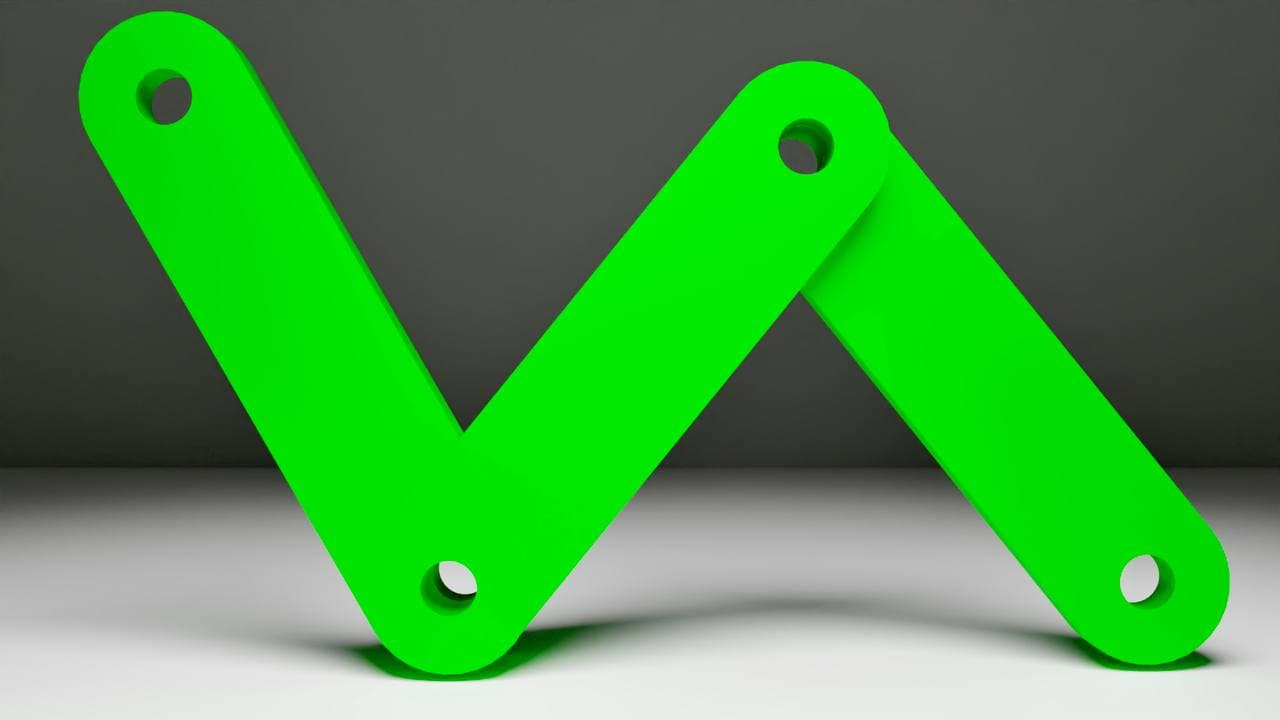
\includegraphics[width=.9\linewidth]{Immagini/Singolarity/3}
		\label{fig:sing4}
	\end{subfigure}
	\begin{subfigure}{.5\textwidth}
		\centering
		% include second image
		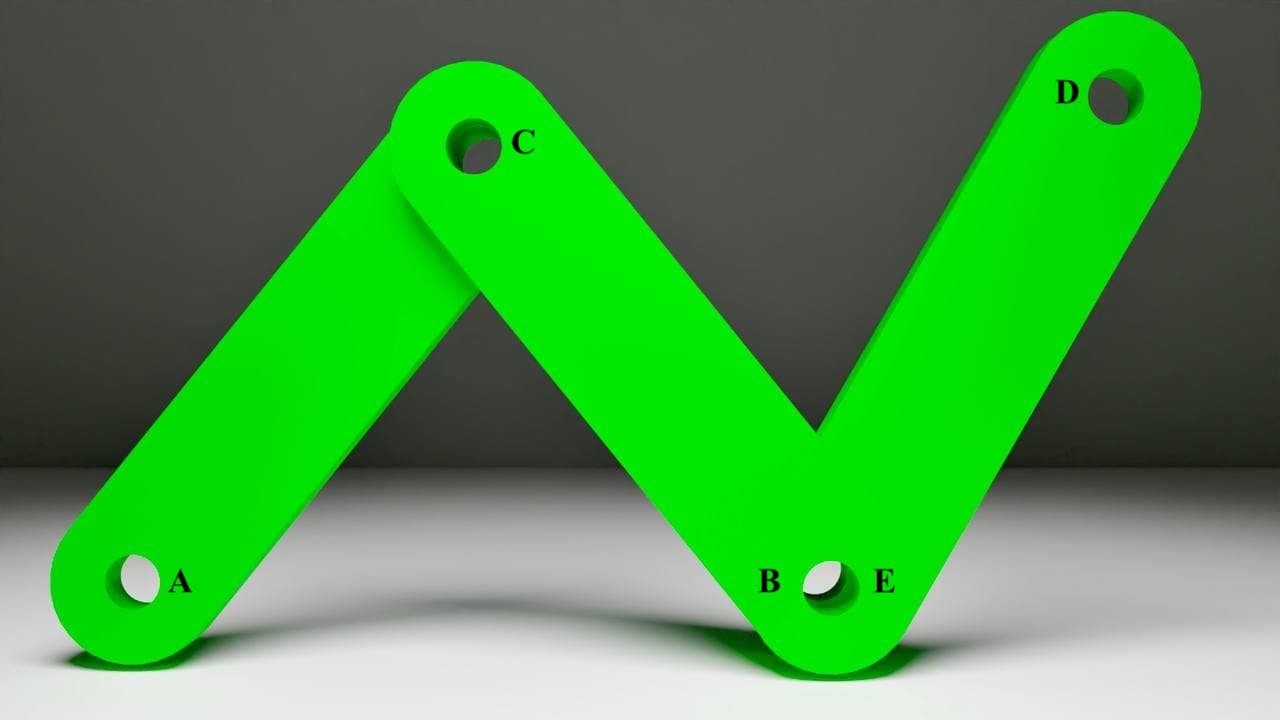
\includegraphics[width=.9\linewidth]{Immagini/Singolarity/4}  
		\label{fig:sing5}
	\end{subfigure}
	\caption{Caso 4 e 5 singolarità}
	\label{Caso4Sing}
\end{figure}
Le soluzioni le possiamo trovare impostando che la lunghezza della x vale nel quarto caso d e nel quinto -d, andando quindi a trovare le soluzioni come:
\begin{equation}
    y_4 = \sqrt{-(x-d)^2}
\end{equation}
e
\begin{equation}
    y_5 = \sqrt{-(x+d)^2}
\end{equation}
Andando ad unire tutti casi visti fino ad ora possiamo vederli visualmente nell'asse $[x,y]$
\begin{figure}[ht]
\begin{center}
    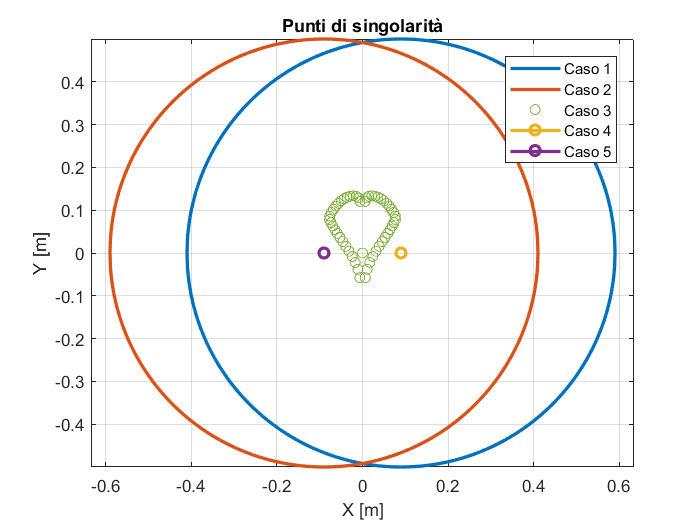
\includegraphics[scale=0.65]{Immagini/Singolarity/SingNew}
    \caption{Punti di singolarità}
    \label{puntiSing}
\end{center}
\end{figure}
\subsection{Manipolabilità}
La manipolabilità ci permette di avere una rappresentazione geometrica delle capacità che ha un punto del nostro sistema. Per andare a calcolarla abbiamo bisogno dell'equazione \ref{eq:J12}, vista nella sezione \ref{sec:CalcoloVelCin}.
\\Andiamo a definire la matrice
\begin{equation}
    J_{man} = JJ^T
\end{equation}
Da questa possiamo ricavare gli autovalori $\Lambda$. Definiamo poi  l'indice di manipolabilità \textbf{r} come:
\begin{equation}
    r = \frac{\max\lambda}{\min\lambda}
\end{equation}
Questo numero può variare tra 1 e $+\infty$, più è piccolo e meno si rischia di andare in singolarità. Possiamo andare a rappresentare il numero di condizionamento tramite i grafici seguenti: 
\begin{figure}[!ht]
	\begin{subfigure}{.55\textwidth}
		\centering
		% include first image
		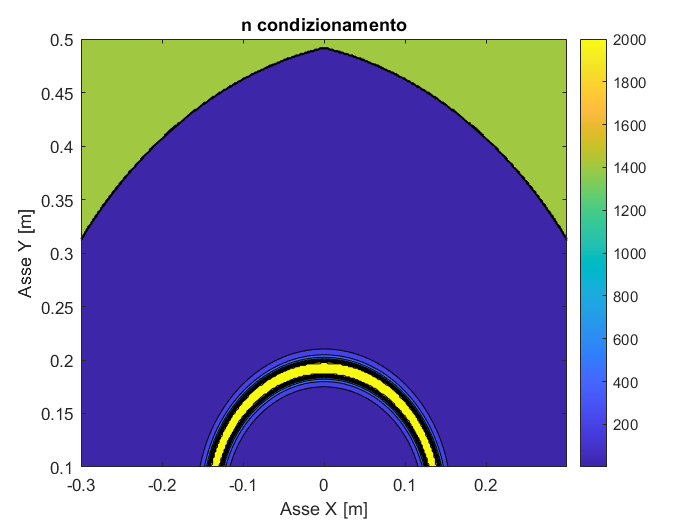
\includegraphics[width=.9\linewidth]{Immagini/Singolarity/Ncond}
		\label{fig:ncond}
	\end{subfigure}
	\begin{subfigure}{.55\textwidth}
		\centering
		% include second image
		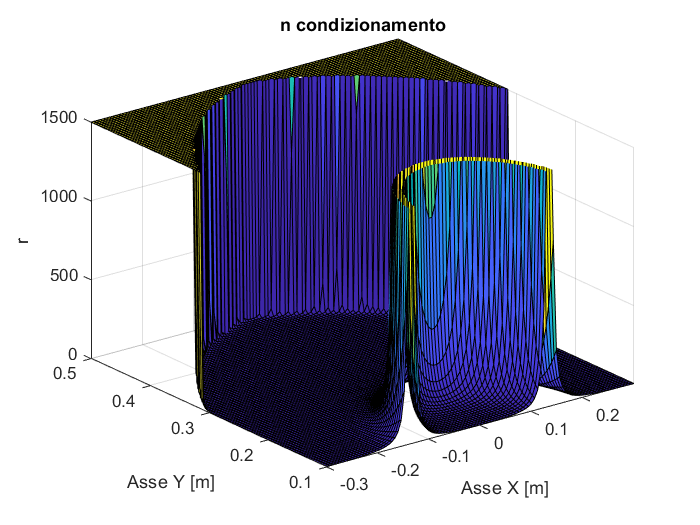
\includegraphics[width=.9\linewidth]{Immagini/Singolarity/Ncond_surf}  
		\label{fig:nconds}
	\end{subfigure}
	\caption{Numero di condizionamento}
	\label{NumCondiz}
\end{figure}
\\Nel primo grafico viene mostrato il piano x,y ed il numero di condizionamento è definito come una colormap, i punti di color blu sono quelli con un r piccolo ed in questi non siamo in condizioni di singolarità, invece quelli tendenti al verde/giallo sono i casi di singolarità che abbiamo visto prima. Nella seconda figura possiamo vedere la stessa rappresentazione però in tre dimensioni, utilizziamo l'asse z per rappresentare il numero di condizionamento; anche qua le zone di singolarità sono chiaramente visibili.
In questo secondo grafico invece andiamo a concentrarci sulla zona di movimentazione ideale del manipolatore, più ci si avvicina allo zero, più il valore di r aumenta, questo per il fatto che stiamo raggiungendo una zona critica.
\subsection{Workspace}
Dalle analisi appena effettuate sui punti di singolarità e sul numero di condizionamento è stato possibile descrivere lo spazio di lavoro del manipolatore. In prima battuta ci si è concentrato sull'analizzare gli angoli di movimentazione dei giunti e i loro vincoli, in particolare il link sinistro con angolo $\theta_1$ avrà una movimentazione di $210^\circ$ al massimo, mentre il link destro con angolo $\theta_2$ ha una movimentazione di $180^\circ$. Questa limitata mobilità è data dai vincoli che ci sono tra le due braccia, infatti, se a livello teorico si possono ottenere configurazioni particolari come quella vista in figura \ref{Caso4Sing} nella pratica non è possibile muovere né manualmente né automaticamente i giunti per ottenere quei casi. Possiamo andare quindi a rappresentare gli angoli di movimentazione mediante la seguente immagine: 
\begin{figure}[ht]
	\begin{center}
		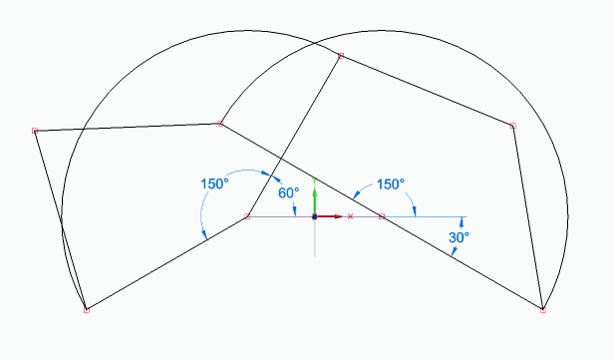
\includegraphics[scale=0.7]{Immagini/Singolarity/workangle}
		\caption{Angoli di movimentazione dei giunti motorizzati}
	\end{center}
\end{figure}
\\Andando ora ad unire gli angoli di movimentazione del manipolatore ed i punti di singolarità, è possibile descrivere lo spazio di lavoro mediante un rettangolo che non viola alcuna condizione
\begin{figure}[ht]
	\begin{center}
		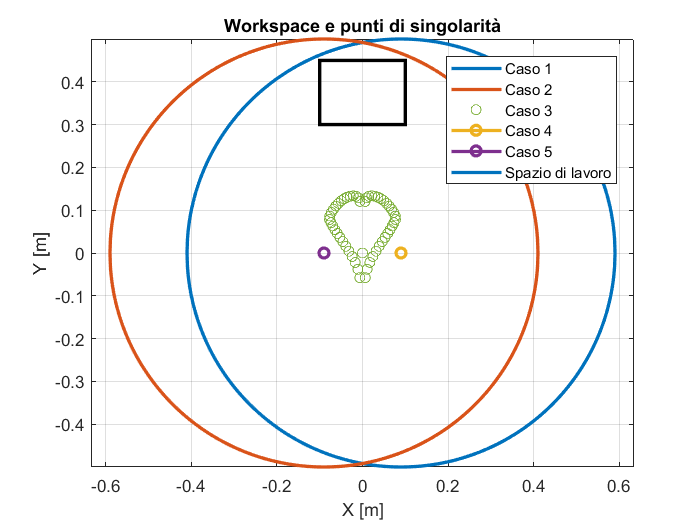
\includegraphics[scale=0.6]{Immagini/Singolarity/Worksing}
		\caption{\textit{Workspace} 5R}
	\end{center}
\end{figure}
\\Successivamente, per verificare che lo spazio di lavoro fosse corretto e rispettasse tutte le condizioni è stata fatta un'analisi sul numero di condizionamento del \textit{workspace}:
\begin{figure}[ht]
	\begin{center}
		\includegraphics[scale=0.6]{Immagini/Singolarity/ncondsl}
		\caption{Numero di condizionamento workspace}
	\end{center}
\end{figure}
\\Su tutto il piano x,y si nota come il numero di condizionamento assume valori bassi, questo implica che non vi è singolarità, gli unici punti critici sono quelli esterni, nei quali il valore è vicino a 6, (comunque minore di $\infty$), questi punti vanno a rappresentare casi nei quali il manipolatore avrà più difficoltà a muoversi, ma non sono veri e propri casi di singolarità.